\documentclass[a4paper]{article} 
\addtolength{\hoffset}{-2.25cm}
\addtolength{\textwidth}{4.5cm}
\addtolength{\voffset}{-3.25cm}
\addtolength{\textheight}{5cm}
\setlength{\parskip}{0pt}
\setlength{\parindent}{0in}

\usepackage[square,sort,comma,numbers]{natbib}
\usepackage{blindtext} % Package to generate dummy text
\usepackage{charter} % Use the Charter font
\usepackage[utf8]{inputenc} % Use UTF-8 encoding
\usepackage{microtype} % Slightly tweak font spacing for aesthetics
\usepackage{amsthm, amsmath, amssymb} % Mathematical typesetting
\usepackage{float} % Improved interface for floating objects
\usepackage{hyperref} % For hyperlinks in the PDF
\usepackage{graphicx} % Enhanced support for graphics
\usepackage{subcaption} % Required for subfigures

\usepackage{xcolor} % Driver-independent color extensions
\usepackage{pseudocode} % Environment for specifying algorithms in a natural way
\usepackage[mmddyy]{datetime} % Uses YEAR-MONTH-DAY format for dates

\usepackage{tikz}

\usepackage{fancyhdr} % Headers and footers
\pagestyle{fancy} % All pages have headers and footers
\fancyhead{}\renewcommand{\headrulewidth}{0pt} % Blank out the default header
\fancyfoot[L]{} % Custom footer text
\fancyfoot[C]{} % Custom footer text
\fancyfoot[R]{\thepage} % Custom footer text
\newcommand{\note}[1]{\marginpar{\scriptsize \textcolor{red}{#1}}} % Enables comments in red on margin

\DeclareMathOperator*{\argmin}{arg\,min}

%----------------------------------------------------------------------------------------


%-------------------------------
%	TITLE VARIABLES (identify your work!)
%-------------------------------

\newcommand{\yourname}{PICARD Emilio} % replace YOURNAME with your name
\newcommand{\youremail}{emilio.picard@free.fr} % replace YOUREMAIL with your email
\newcommand{\assignmentnumber}{1} % replace X with the lab session number

\begin{document}

%-------------------------------
%	TITLE SECTION (do not modify unless you really need to)
%-------------------------------
\fancyhead[C]{}
\hrule \medskip
\begin{minipage}{0.295\textwidth} 
\raggedright
\footnotesize
\yourname \hfill\\
\youremail
\end{minipage}
\begin{minipage}{0.4\textwidth} 
\centering 
\large 
Lab session \# \assignmentnumber\\ 
\normalsize 
ALTEGRAD 2023\\ 
\end{minipage}
\begin{minipage}{0.295\textwidth} 
\raggedleft
\today\hfill\\
\end{minipage}
\medskip\hrule 
\bigskip

%-------------------------------
%	ASSIGNMENT CONTENT (add your responses)
%-------------------------------

\section{Question 1}

\noindent
The basic self-attention mechanism is a common approach to capture the semantic representation
of words. It typically relies on creating a single attention vector, but this approach can be
limited when applied to tasks such as sentiment classification, as it lacks
sufficient input variety to capture diverse aspects of the sentence.
\\
\\
\noindent
One approach to enhance the basic self-attention mechanism is to incorporate a max or
average pooling layer over all time steps in the forward path. This can help aggregate
features across time steps, but it might be challenging to implement within an RNN-based
architecture, particularly when managing long sequences.
\\
\\
\noindent
A more effective improvement can be achieved by modifying the input to the attention mechanism.
For instance, instead of using a unidirectional approach, a bidirectional LSTM can
be employed to produce a richer representation. This allows the attention mechanism to operate on a more informative
representation, capturing both forward and backward dependencies in the sentence.
\\
\\
\noindent
Furthermore, a known issue with basic self-attention is its tendency to focus on redundant
information, where multiple attention heads may concentrate on the same parts of
the input. To address this, Lin et al. (2017) \cite{Lin} introduced a structured self-attentive mechanism that
includes a penalization term. This term, based on the Frobenius norm, encourages the
attention heads to focus on different parts of the sentence, promoting diversity and leading
to more comprehensive sentence representations.
\\
\\
\noindent
Incorporating these enhancements, such as bidirectional context and penalization for
redundancy, can significantly improve the performance of the basic self-attention mechanism.


\section{Question 2}
\noindent
According to the paper \cite{vaswani2023attentionneed}, The motivations for this
change were leaded in addressing several limitations of recurrent models, particularly for
tasks like machine translation and other sequence-based problems.
\\
\\
\noindent
Recurrent models process sequences sequentially, meaning each time step depends on the previous
one. This limits parallelism and can lead to inefficiencies, especially with long sequences.
Self-attention allows the model to process all tokens in the input sequence simultaneously,
leading to faster computations.
\\
\\
\noindent
Furthermore, In contrast to RNNs, where each time step must wait for the computation
of the previous one, self-attention enables parallel processing of tokens, significantly
speeding up training and inference times. This is especially beneficial for tasks like
machine translation, where large datasets are involved.
\\
\\
\noindent
Additionnaly, Recurrent models often struggle with capturing long-range
dependencies in sequences, as the information has to pass through multiple
time steps, leading to vanishing or exploding gradient problems. Self-attention
directly connects every token with every other token in the sequence, making it easier
to capture dependencies over long distances.
\\
\\
\noindent
Transformers also reduced computational complexity, thanks to self-attention. Finally,
RNNs and LSTMs can suffer from gradient vanishing or exploding when processing long sequences,
making it difficult to learn long-range patterns. Self-attention mitigates this issue by
enabling shorter and more direct paths for gradient flow during backpropagation, improving
training stability.


\section{Bonus (\textit{purpose of my\_patience parameter})}
\noindent
In the context of training a neural network, the \texttt{my\_patience} variable refers to
the patience parameter used in early stopping during training. Early stopping is a
technique used to prevent overfitting and stop training when a model’s performance on
the validation set stops improving. It can prevent also from overfitting.


\section{Training process}
\noindent
I have trained the Hierarchical Attention Network during \texttt{$15$ epochs}.
The hyperparameters can be seen in the notebook.
\\
\\
\noindent
\begin{figure}[H]
    \centering
    \begin{subfigure}[b]{0.45\textwidth}
        \centering
        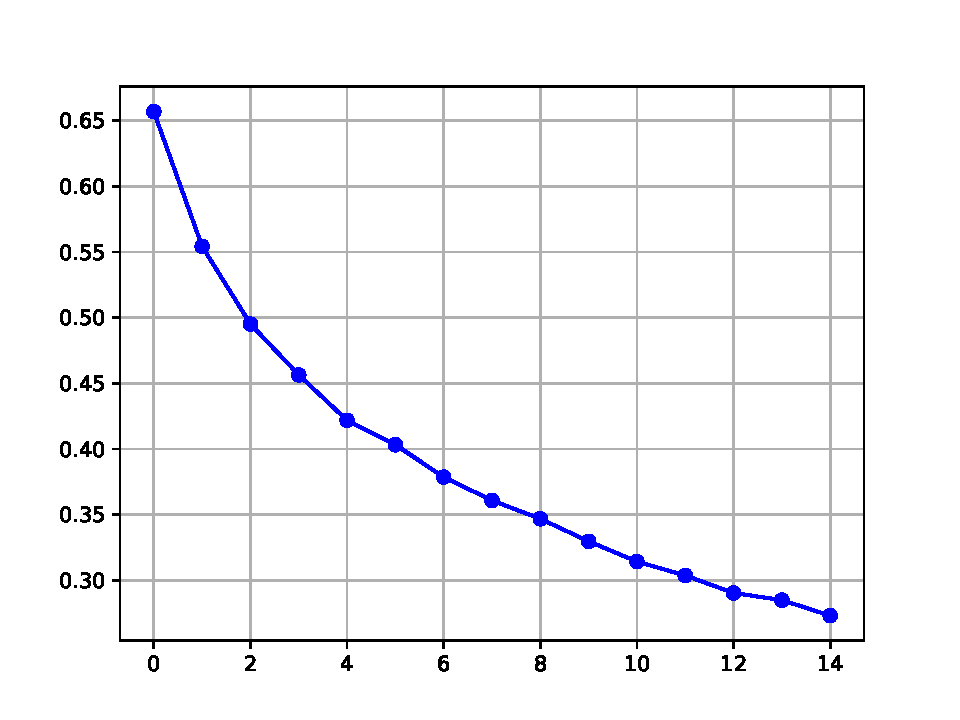
\includegraphics[width=\textwidth]{../figures/train_loss.pdf}
        \caption{train losses over epochs.}
        \label{fig:image1}
    \end{subfigure}
    \hfill
    \begin{subfigure}[b]{0.45\textwidth}
        \centering
        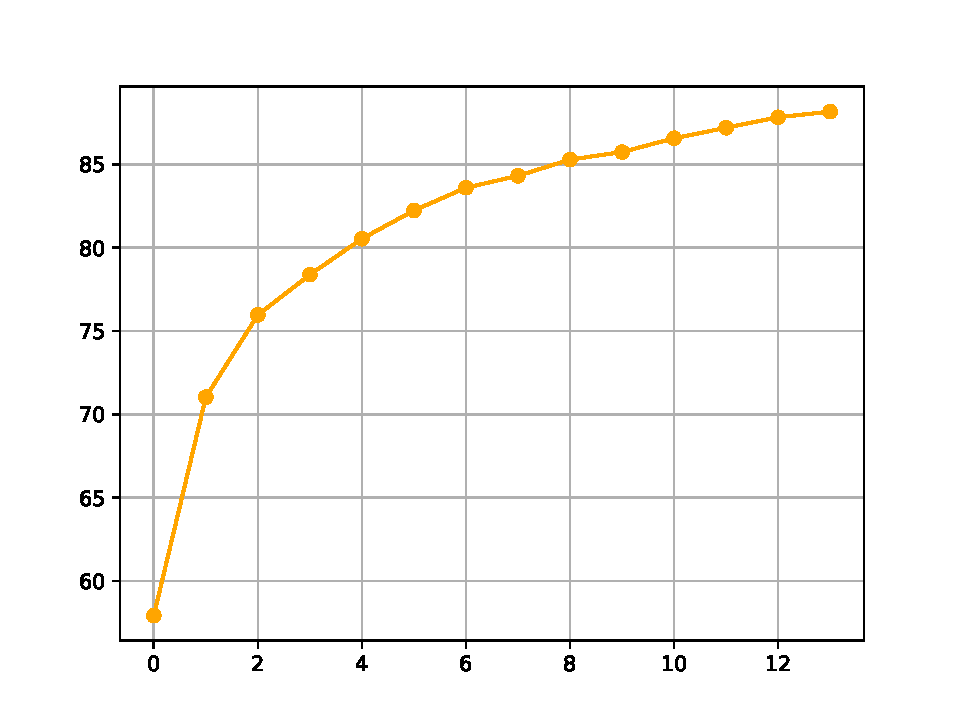
\includegraphics[width=\textwidth]{../figures/train_accs.pdf}
        \caption{train accuracies over epochs.}
        \label{fig:image2}
    \end{subfigure}
    \caption{train accuracies and losses during training, with $15$ epochs.}
    \label{fig:images}
\end{figure}

\begin{figure}[H]
    \centering
    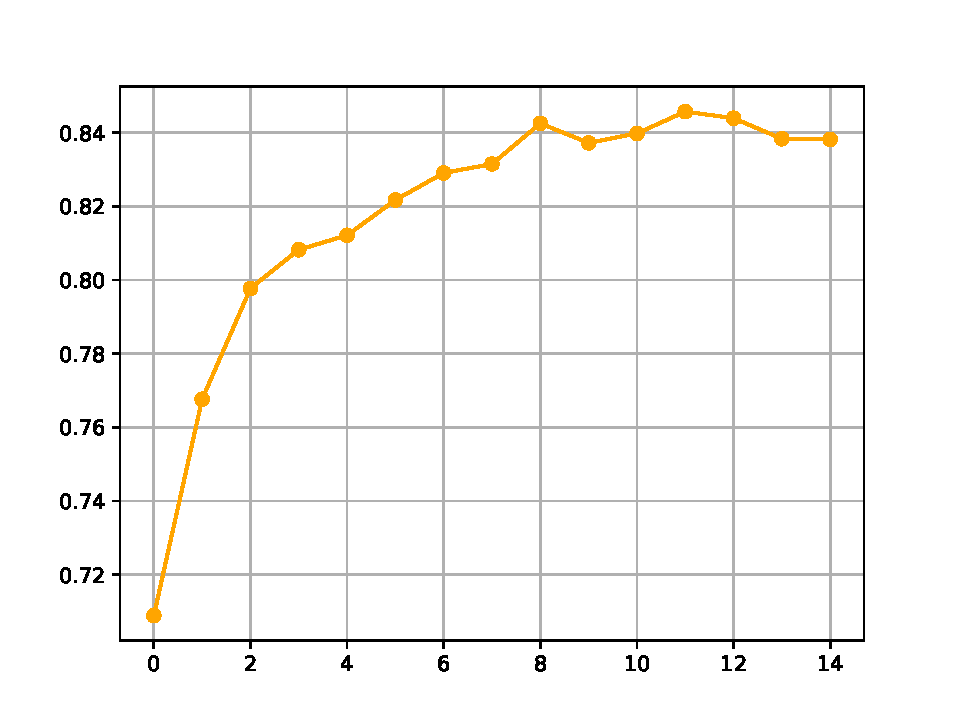
\includegraphics[width=.5\linewidth]{../figures/val_accs.pdf}
    \caption{validation accuracies over epochs.}
    \label{fig:third_image}
\end{figure}
We can see figure \ref{fig:images} the train losses and accuracies during training, wich demonstrate a good
training process.
\\
We can also observe figure \ref{fig:third_image} the validation accuracies over the epochs.



\section{Question 3}
\noindent
For this question, I selected the last document from the test dataset, where the model predicts
it to be a positive ("yes") review. The sentence attention scores (Figure \ref{sentence-scores})
show that certain sentences are given higher weight, likely because they express clear positive
sentiment. For example, sentences like \textit{"a masterpiece"} or either \textit{"[...] downright brillant"}
are prioritized by the model, as they play a key role in forming the positive classification.
\\
\\
\noindent
The word attention scores (Figure \ref{word-scores}) for the sentence \textit{":) First of all, Mulholland Drive 
is downright brillant."} highlight words such
as "downright" or "brillant," which strongly contribute to the positive sentiment if they are putting together.
\\
\\
\noindent
In conclusion, both sentence- and word-level attention scores indicate that the model identifies
the most sentiment-relevant portions of the review, which explains its prediction of a
positive ("yes") classification.


\begin{figure}[H]
    \centering
    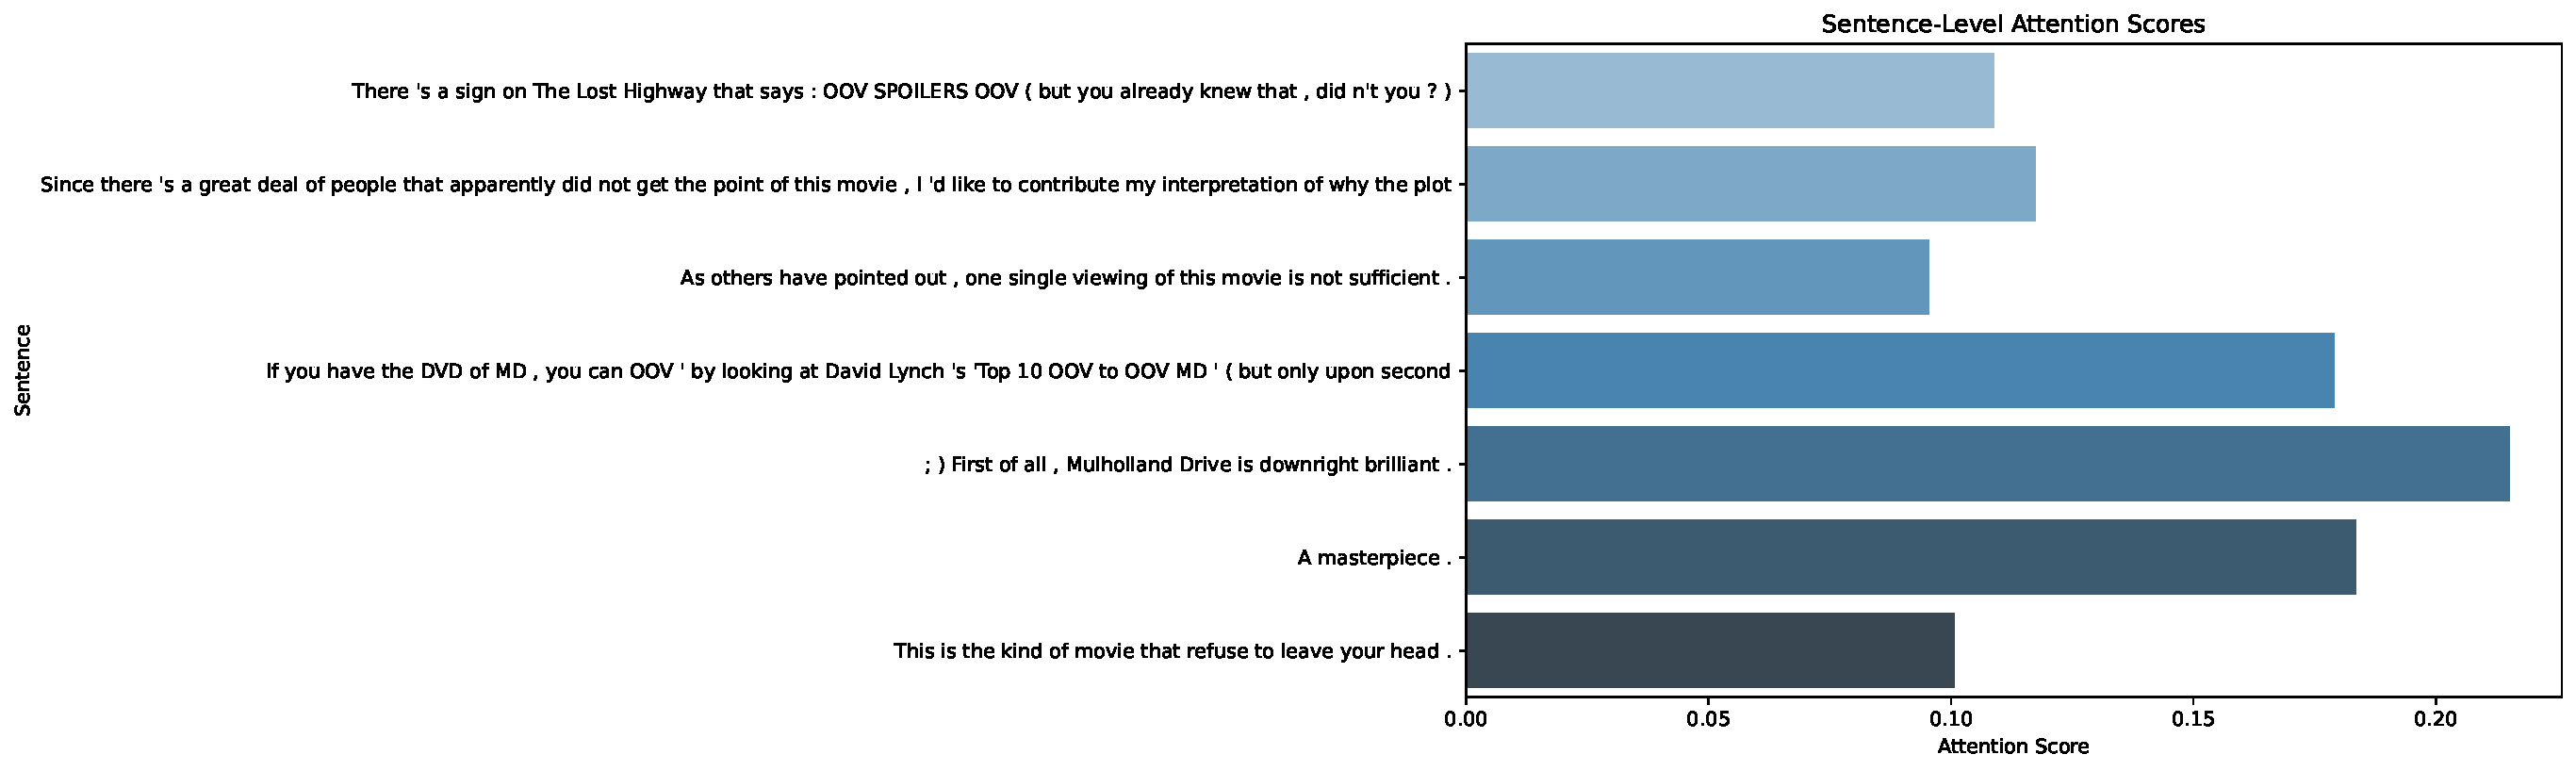
\includegraphics[width=.9\linewidth]{../figures/Sentence_attention_scores.pdf}
    \caption{Sentence attention scores for the last document of the test dataset.}
    \label{sentence-scores}    
\end{figure}

\begin{figure}[H]
    \centering
    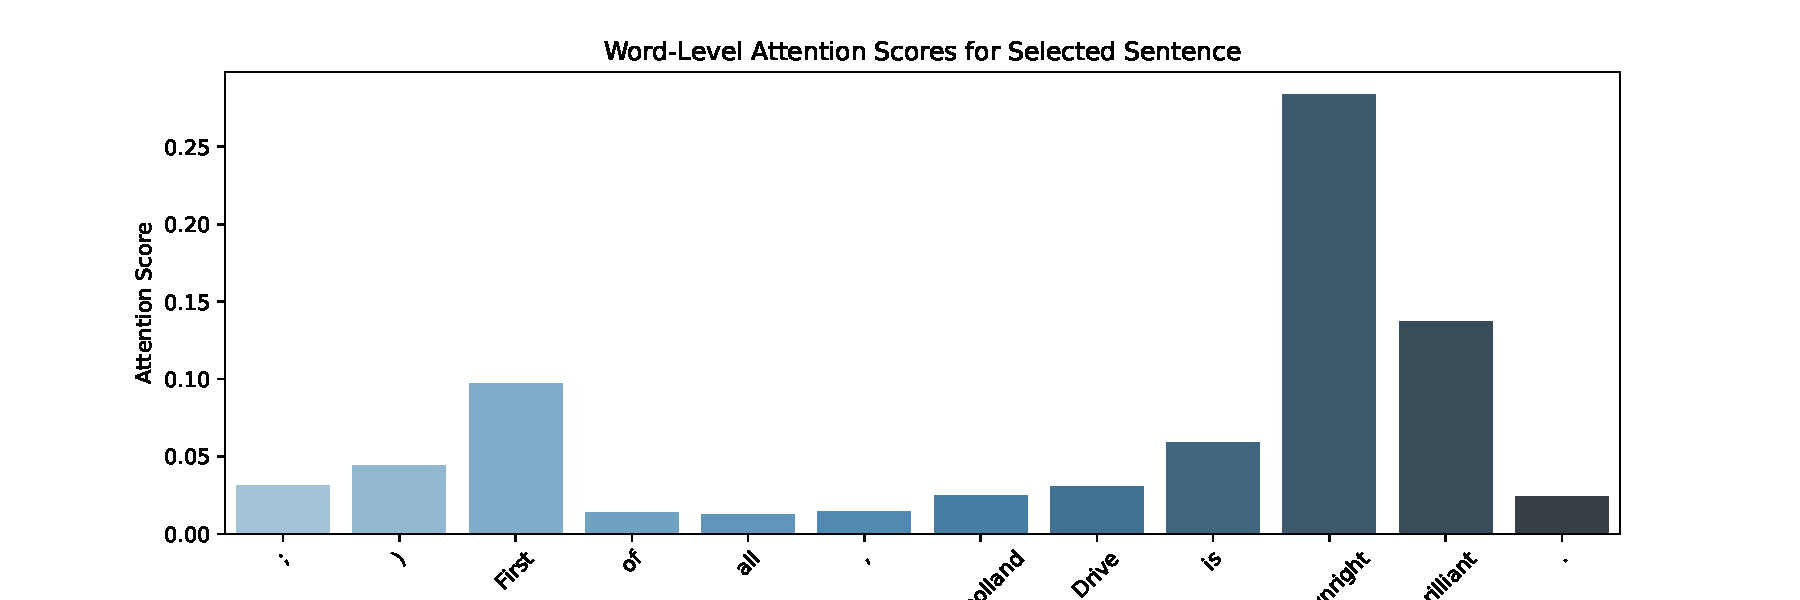
\includegraphics[width=.7\linewidth]{../figures/word_attention_scores.pdf}
    \caption{Word attention scores for the last sentence of the last document of the test dataset.}
    \label{word-scores}    
\end{figure}

\section{Question 4}
\noindent
According to the article \cite{remy2019bidirectionalcontextawarehierarchicalattention}, Hierarchical Attention
Networks (HAN) have several limitations related to both architecture and training.
\\
Firstly, the model processes sentences independently during the initial step of the architecture. This means
that while one sentence is being analyzed, the model ignores other sentences, which can hinder its
ability to capture the overall meaning of the document. As a result, the model may struggle with
understanding context and relationships between sentences.
\\
Additionally, the embedding representation for each sentence is uniform across all instances, which
limits the extraction of diverse and complementary information. By not differentiating embeddings
for various instances, HAN may miss important nuances that could enhance the model's performance
on document understanding tasks.


%------------------------------------------------

\bibliographystyle{plain}
\bibliography{references} % citation records are in the references.bib document

\end{document}
